%%%%%%%
\subsection{Utilization-based resource quota comparison}\label{s:Evaluation:ResourceOptimal}

% \todo{Experiments with task agglomeration and scheduling against a solution with optimal resource quotas}

The last scenario in the experimental process revolves around the optimal utilization of available node resources.
In previous scenarios, it has been assumed that each container is assigned a single processor.
This may have not fully reflected the capabilities of container computing as pods can have assigned partial resource quotas as well. 
This scenario has been prepared to make sure the performance of the default solution was not unintentionally affected in previous runs.
To compare the results from both scenarios, the Montage2-v1.0 workflow has been considered for this experiment.

As each pod in Kubernetes can have different resource quotas, it has been decided to adjust them to the values from appropriate measurements, based on the operation that is run by the tasks in this specific container.
Those measurements concentrate only on the CPU utilization, since any possible slowdown may have been caused only by improper management of this single resource.
In \cref{tab:res-util:setup} both the average usages measured and the actual assigned values are provided.
Some of the tasks have a reported utilization rate of zero, and to make a pod creation possible, a minimum CPU request has been introduced with two different values provided for this scenario.


% Tabelka z metrykami - Montage-1.0
\begin{table}[H]
    \centering
    \begin{tabular}{|c|c|c|c|c|}
    \cline{1-5}
        \multirow{2}{*}{Operation name} 
        &
        \multicolumn{2}{|c|}{Measured CPU usage}
        &
        \multicolumn{2}{|c|}{Assigned CPU request}  \\
    \cline{2-5}
        & m5.xlarge & m5a.xlarge & min CPU = 0.25 & min CPU = 0.50 \\
    \cline{1-5}
        mProject & 0.95 & 0.95 & \multicolumn{2}{|c|}{0.95} \\
    \cline{1-5}
        mDiffFit & 0.0 (!) & 0.0 (!) & 0.25 & 0.50 \\
    \cline{1-5}
        mConcatFit & 0.82 & 0.77 & \multicolumn{2}{|c|}{0.85} \\
    \cline{1-5}
        mBgModel & 1.00 & 1.00 & \multicolumn{2}{|c|}{1.00} \\
    \cline{1-5}
        mBackground & 0.0 (!) & 0.20 & 0.25 & 0.50 \\
    \cline{1-5}
        mImgtbl & 0.44 & 0.60 & \multicolumn{2}{|c|}{0.60} \\
    \cline{1-5}
        mAdd & 0.76 & 0.78 & \multicolumn{2}{|c|}{0.8} \\
    \cline{1-5}
        mViewer & 1.00 & 1.00 & \multicolumn{2}{|c|}{1.00} \\
    \cline{1-5}
    \end{tabular}
    \caption{Usages and CPU requests per workflow operation}
    \label{tab:res-util:setup}
\end{table}
%%%%


The execution traces for both setups are presented in \cref{fig:evaluation:res-util:m10:plugin}.
Adjusting CPU requests for pods resulted in an execution of up to six pods in parallel on nodes with only 4 vCPUs.
For a setup with a minimal CPU request of 0.5 vCPU, the utilization is nearly the same as with fixed CPU requests -- the parallelization of five pods occurs rarely and for a short time.
Only the other setup seems to really benefit from usage-based configuration.


%%%%%%%% Traces - Optimal
\begin{figure}[H]
\begin{subfigure}{1.0\textwidth}
\centering
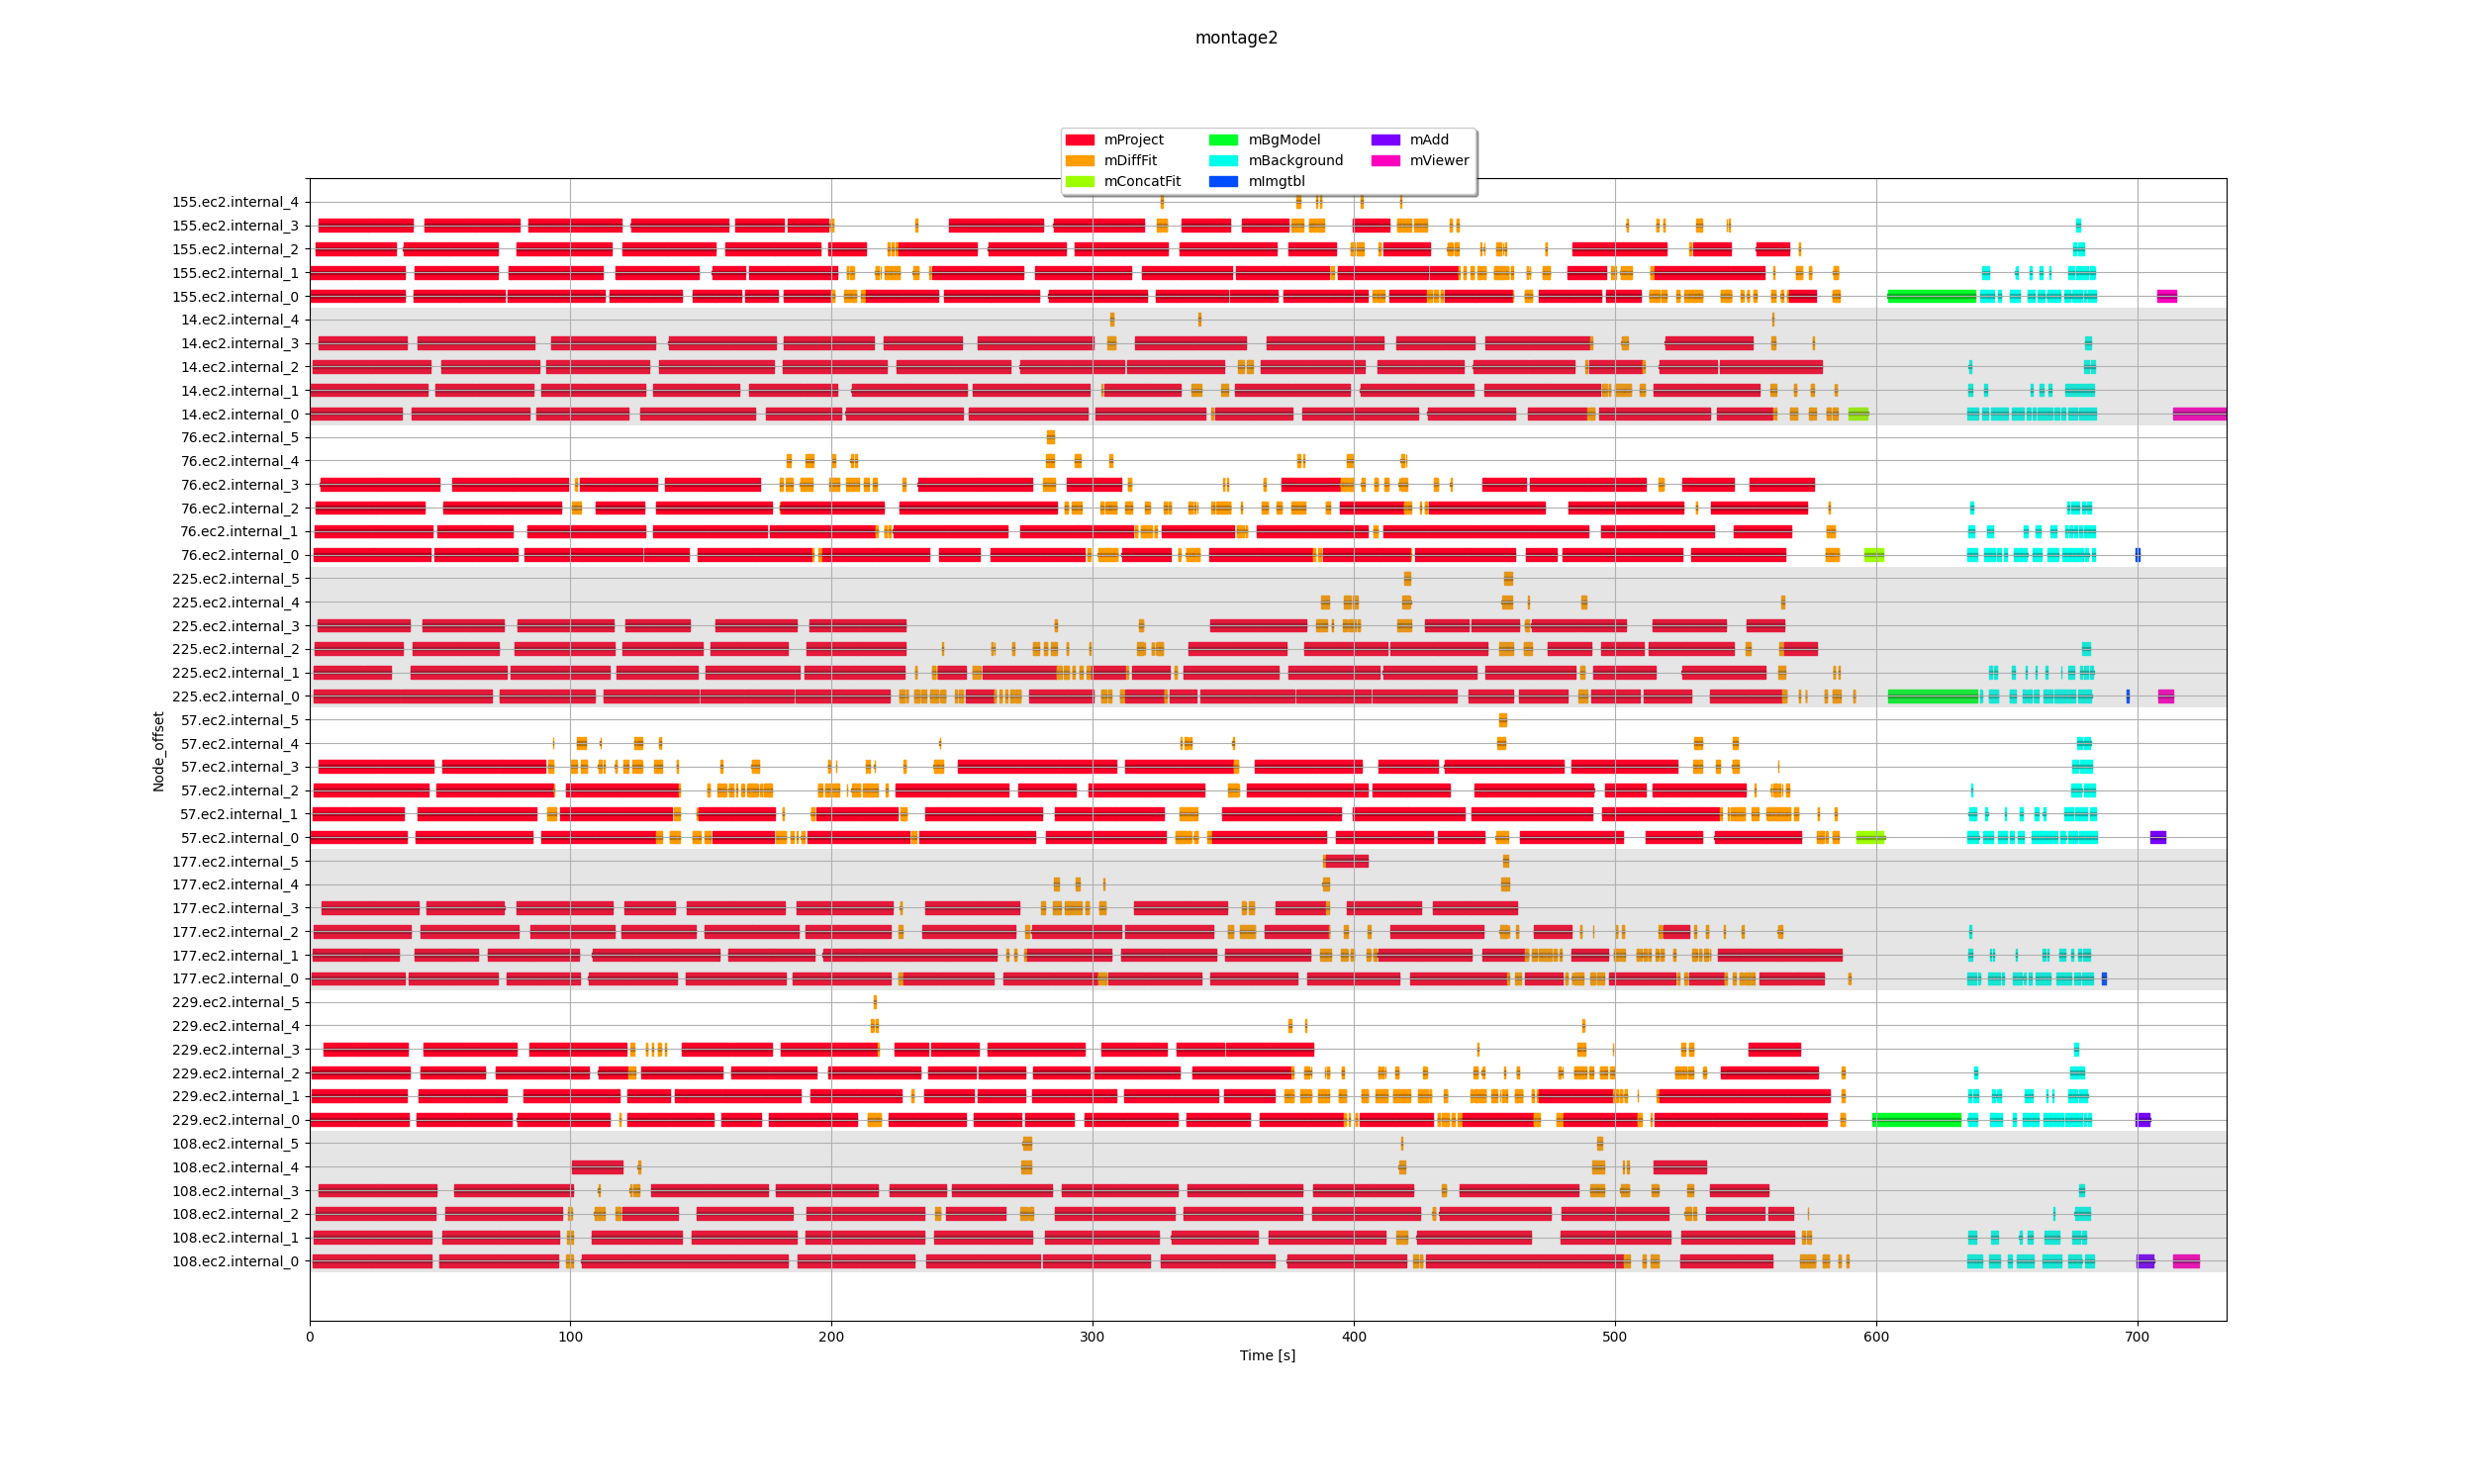
\includegraphics[width=1\linewidth]{figures/6-3-m1.0-optimal-cpu-0.25.png}
\caption[Selected example execution trace of Montage2-v1.0 with usage based CPU requests, min 0.25]{min CPU = 0.25}
\label{fig:evaluation:res-util:m10:025}
\end{subfigure}
\begin{subfigure}{1.0\textwidth}
\centering
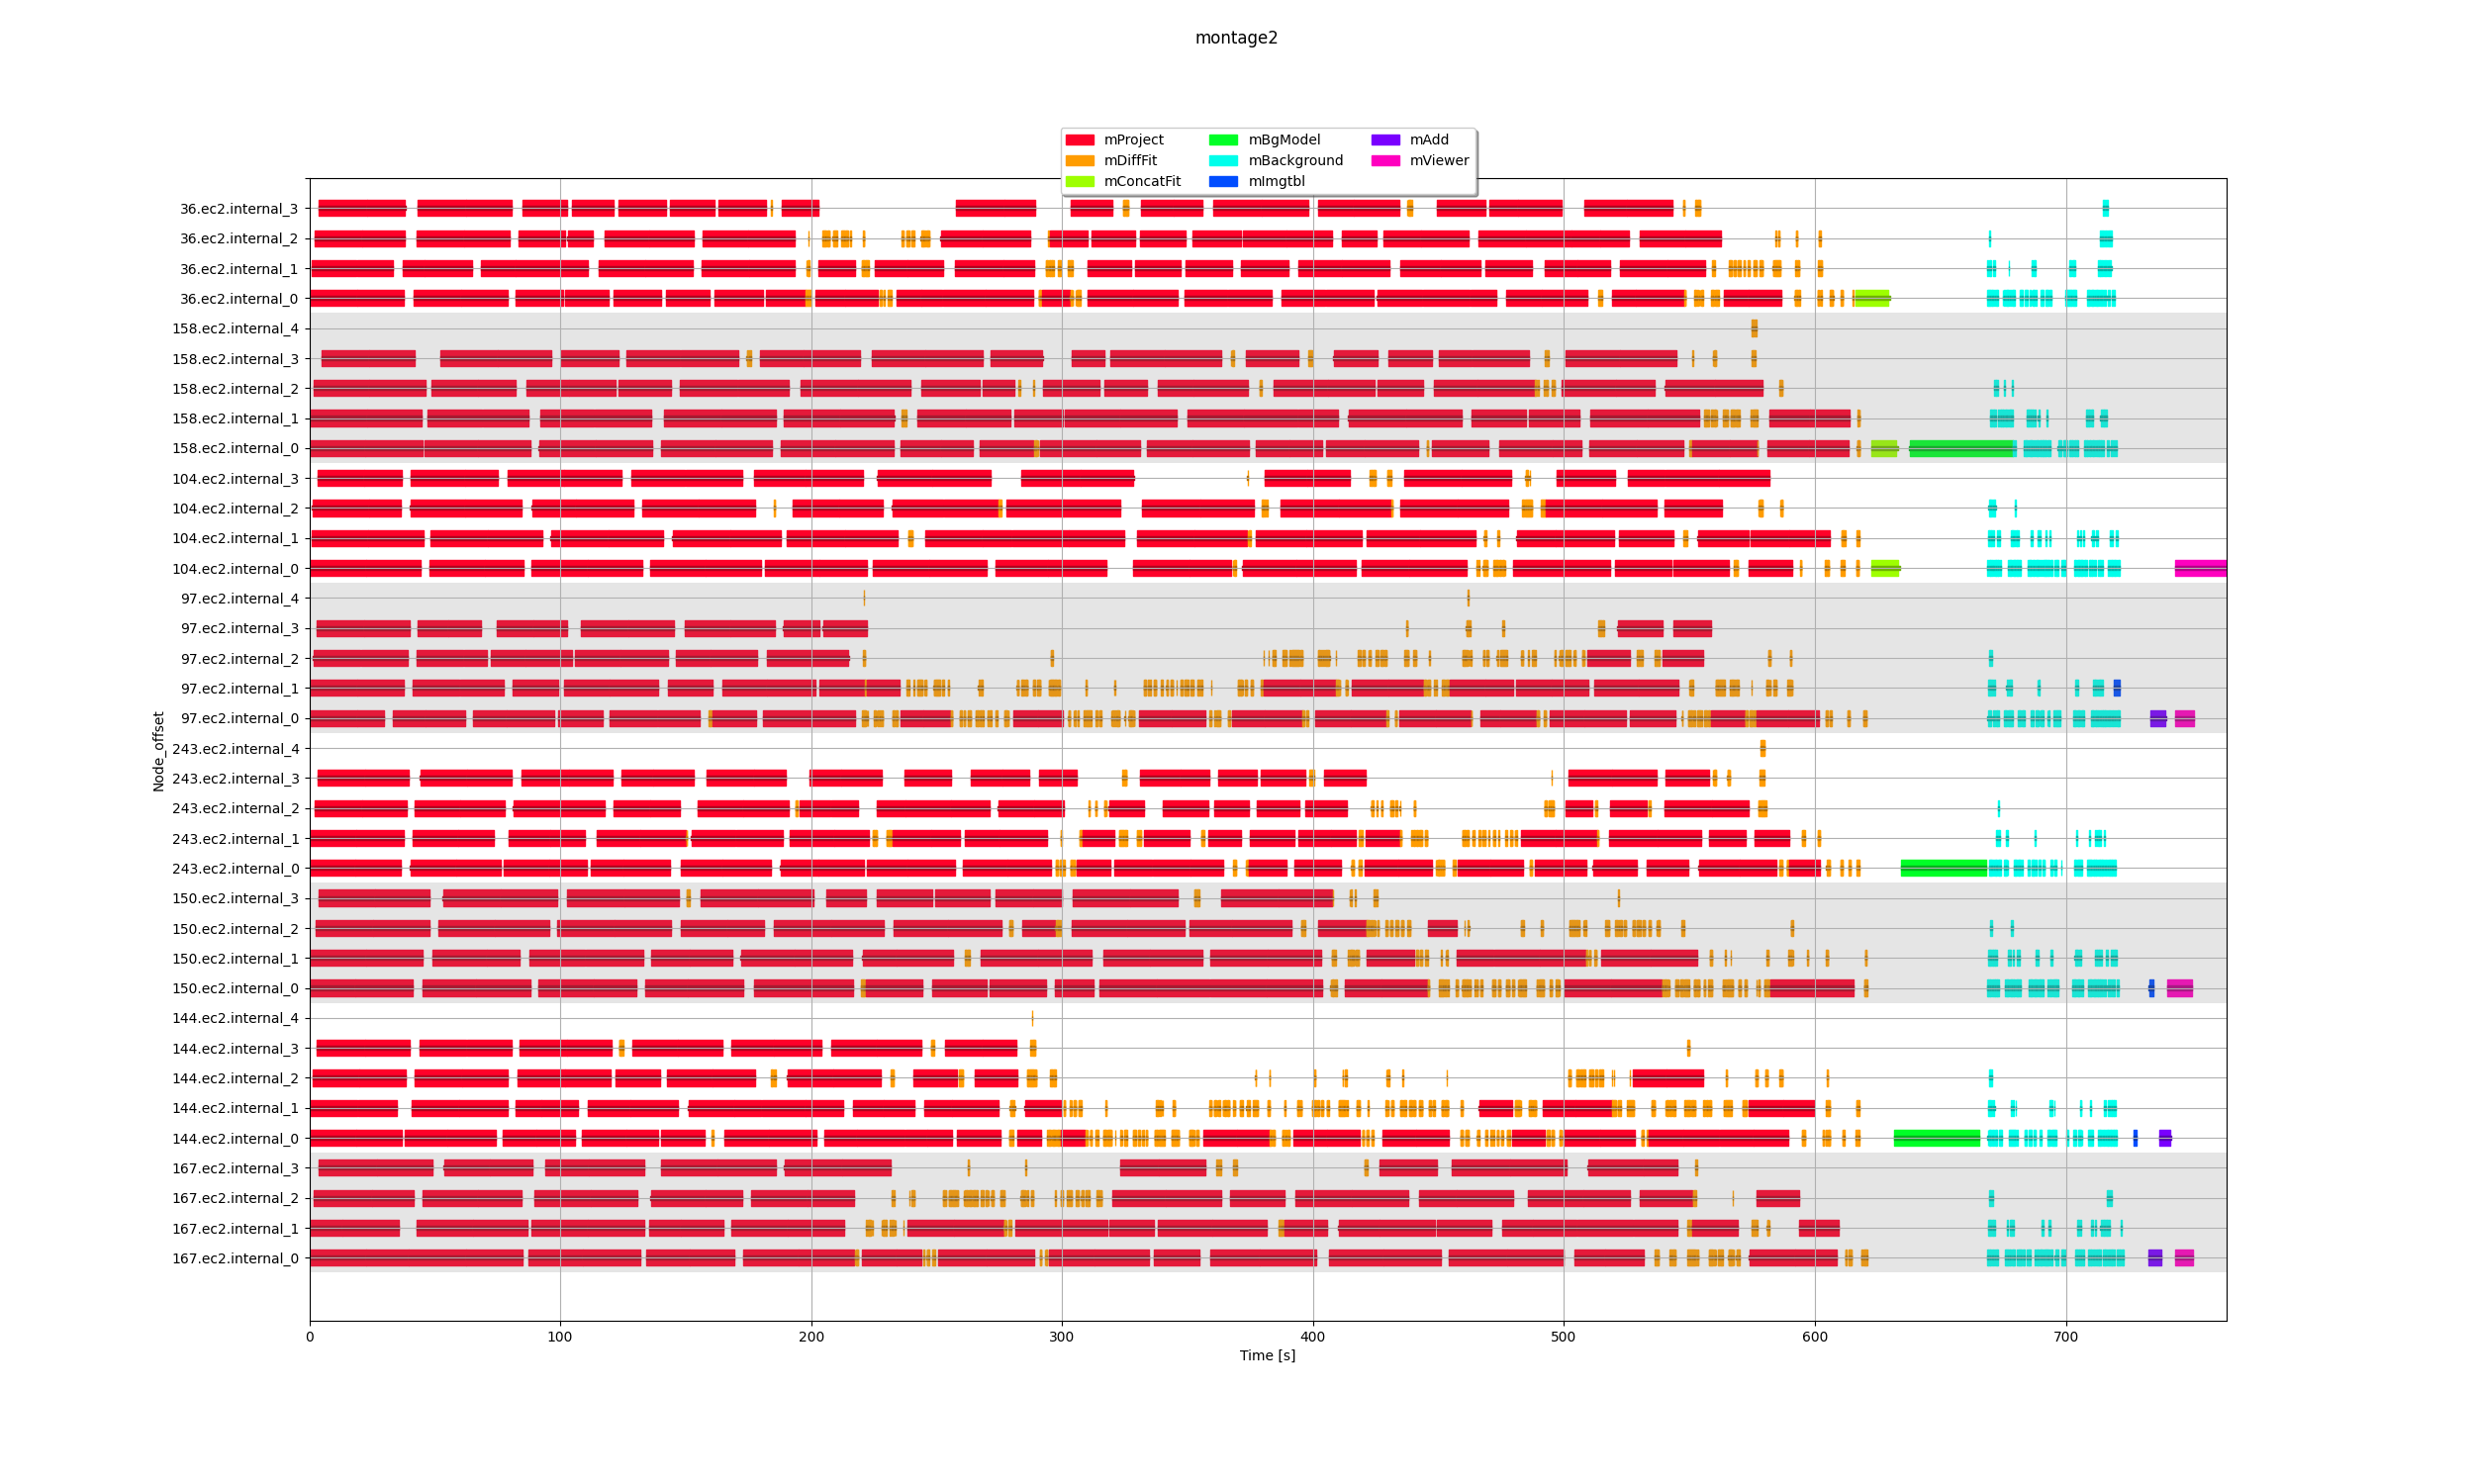
\includegraphics[width=1\linewidth]{figures/6-3-m1.0-optimal-cpu-0.50.png}
\caption[Selected example execution trace of Montage2-v1.0 with usage based CPU requests, min 0.50]{min CPU = 0.50}
\label{fig:evaluation:res-util:m10:050}
\end{subfigure}
\centering
%%
\caption[Selected example execution traces of Montage2-v1.0 with usage based CPU requests]{Selected example execution traces of Montage2-v1.0 with usage based CPU requests.}
\label{fig:evaluation:res-util:m10:plugin}
\end{figure}
%%%%%%%%


With the metrics provided in \cref{tab:res-util:results} it can be concluded that the final performance is highly dependant on the minimal CPU request.
It would, however, require to check all possible configurations to verify which setup performs the best with no guarantee for better results.


%%% Tabelka z metrykami - Optimal
\begin{table}[H]
    \centering
    \begin{tabular}{|c|c|c|c|c|c|}
    \cline{1-6}
        \multirow{2}{*}{Scenario} 
        &
        \multirow{2}{*}{Approach} 
        &
        \multicolumn{4}{|c|}{Metrics} \\
    \cline{3-6}
        & & Makespan & Job slowdown & SLR & CO \\
    \cline{1-6}
        \multirow{2}{*}{\vtop{\hbox{\strut\centering usage-based}\hbox{\strut\centering CPU requests}}} & min CPU = 0.25 & 746.7 & 48 & 7.27 & 12176 \\
    \cline{2-6}
        & min CPU = 0.50 & 779.1 & 243 & 7.55 & 15083 \\
    \cline{1-6}
        \multirow{3}{*}{\vtop{\hbox{\strut\centering fixed}\hbox{\strut\centering CPU requests}}} & kube-scheduler & 778.5 & 537 & 7.61 & 8200 \\
    \cline{2-6}
        & HEFT + kube-scheduler & 711.9 & 239 & 7.08 & 1271 \\
    \cline{2-6}
        & PEFT + kube-scheduler & 770.2 & 256 & 7.31 & 2008 \\
    \cline{1-6}
    \end{tabular}
    \caption{Comparison of metrics from Montage2-v1.0 execution from both scenarios}
    \label{tab:res-util:results}
\end{table}
%%%

The overall best solution for task clustering of all is still the HEFT schedule-based one.
For both utilization-based setups, the one with minimal CPU request set to 0.25 results in the better workflow execution efficiency.
It performs over 3\% better in terms of makespan reduction than PEFT and the default solution with fixed CPU requests.
Nonetheless, it is still behind the HEFT one, which has almost 5\% shorter execution times.


On the other hand, the utilization-based approach seems to achieve much better job slowdown.
As there is a higher chance for a pod to match its quota with the available resources in the cluster, the difference between time of arrival and time of task execution start lowers on average.
The only downside seems to be a higher containerization overhead, which seems to be one of the crucial aspects affecting the performance of this approach.
There is definitely a potential of improving the overall effectiveness of usage-based solutions if the lesser CO is achieved.
